\documentclass[11pt]{article}
\usepackage[margin=1in]{geometry}
\usepackage{amsmath,amssymb,booktabs,graphicx}
\usepackage[hidelinks]{hyperref}
\usepackage{xurl}
\setlength{\emergencystretch}{2em}
\newtheorem{proposition}{Proposition}
\newenvironment{proof}{\par\noindent\textit{Proof.}\ }{\hfill\textit{Q.E.D.}\par}
\title{AFTER: Digital Twins for Cyberattack and Recovery Monitoring in Industrial Robots}
\author{Muhammad Usman \and Haiqa Mushtaq}
\date{17 October 2026}
\begin{document}
\maketitle
\begin{abstract}
An anomaly alarm can remain active after a robot recovers, or clear while an unauthorized motion deviation persists. Model mismatch complicates both decisions. We distinguish proximity to a nominal twin from proximity to the motion the same plant would have followed without command corruption. Conditional error bounds expose a clearance-feasibility constraint: if reference uncertainty exceeds the permitted recovery tolerance, no observation can satisfy the proposed return certificate. We test a command-driven reference fitted during clean commissioning, thirteen detection and clearance rules, and paired-plant recovery measurements in a prospectively frozen simulation of 216 episodes. The uncertainty-aware return candidate reduced benign alarm observations from 621 to 309 relative to nominal fixed return, but cleared within five seconds in only 36 of 108 detected events with physical return. Its primary improvement criterion failed. Removing the uncertainty allowance at the same entry threshold reduced benign alarms further, to 140, and restored clearance in all 108 events without observed premature clearing. Nominal-reference and paired-plant return times differed in 21 of 135 intervention episodes. These findings identify a failure mode of the tested clearance design and show why reduced nuisance alarms alone cannot establish a recovery benefit. They support a normal-operation clearance-feasibility check before confirmatory attack evaluation; they do not establish a novel detector or physical safety guarantee.
\end{abstract}
\noindent\textbf{Keywords:} digital twin; robotic cybersecurity; alarm recovery; model mismatch; counterfactual evaluation.

\section{Introduction}
A motion detector answers whether an observation departs from expected behavior. Clearing its alarm asks a different question: whether the condition that justified retaining the alarm has ended. A small prediction residual can arise because a predictor follows the perturbed motion. Conversely, an uncorrected reference can remain displaced from legitimate motion because its plant model is inaccurate.

This distinction matters when evaluating a digital twin for robotic attack monitoring. Restoring an approved command does not instantly remove the motion caused by a preceding corrupted command. Nor does returning near a nominal model necessarily mean returning to the trajectory of the actual plant. We study these quantities separately, using protected approved commands and truthful noisy joint measurements.

The analysis makes three bounded contributions. First, it states the conditions under which reference discrepancy can bound attack-induced motion discrepancy, including a case in which clearance is impossible. Second, it defines an evaluator-only paired-plant reference that avoids using the detector's model as recovery truth. Third, it reports a frozen comparison of commissioning-based references and clearance rules, including a failed proposed improvement and a stronger matched control. System identification, interval reasoning and dwell logic are established ingredients; the study makes no first-of-its-kind claim for their combination.

\section{Related work and comparison scope}
CASPER and its edge-computing successor detect robotic motion anomalies from external inertial measurements~\cite{casper,edge}. Their sensor modality and published experiment differ from the joint-state and approved-command simulation here. Our earlier IMU predictor experiments remain a separate track; their weights and published attack scores are not transferred into this comparison.

FAIL-Detect calibrates failure-monitoring bands from successful robot rollouts~\cite{fail}. We use an independently implemented constant-band threshold component on the common reference-discrepancy score, with an explicit finite-sample rank. This is a restricted comparison, not a reproduction of its learned scores, robot policies or complete experiments. Source inspection distinguishes the sign printed in the arXiv v1 appendix from the executable functional predictor, which uses the appropriate upper-tail sign. We therefore do not attribute that printed discrepancy to failure of the released method.

RESCUE evaluates whether alarms enable beneficial interventions by branching robot-policy simulations~\cite{rescue}. Our target is whether the motion effect of command corruption has ended, rather than which intervention should be taken. Counterfactual recovery evaluation itself is already represented in that work. Interval observers likewise address model uncertainty in fault detection~\cite{interval}. RAPIO and recent digital-twin FDI work are close recovery-related leads~\cite{rapio,kaisar}; their full method-to-code correspondence remains unresolved in our source audit. They are not presented as reproduced or defeated baselines.

\section{Recovery target and conditional bounds}
Let $x_t$ be the perturbed plant state and $x_t^0$ the state of the same plant under the complete approved command history without corruption. The monitor receives $y_t=x_t+n_t$ and maintains a reference $r_t$. For positive training scales $s_j$, define
\begin{equation}
 \|v\|_s=\max_j |v_j|/s_j,\qquad
 d_t=\|x_t-x_t^0\|_s,\qquad c_t=\|y_t-r_t\|_s.
\end{equation}
The evaluator uses $d_t$; the monitor can compute $c_t$. With noise absent, $x_t=r_t\ne x_t^0$ gives $c_t=0$ but $d_t>0$. Conversely, $x_t=x_t^0\ne r_t$ gives $d_t=0$ but $c_t>0$. Reference proximity and recovery are therefore not interchangeable without an assumption linking the reference to the uncorrupted plant.

\begin{proposition}
If $\|x_t^0-r_t\|_s\le b_t$ and $\|n_t\|_s\le\eta_t$, then
\begin{equation}
 \max(0,c_t-b_t-\eta_t)\le d_t\le c_t+b_t+\eta_t.
\end{equation}
\end{proposition}
\begin{proof}
Write $x_t-x_t^0=(y_t-r_t)-n_t-(x_t^0-r_t)$ and apply the triangle inequality and reverse triangle inequality. Aligned scalar errors attain the bounds, so they cannot generally be tightened from these scalar allowances alone.
\end{proof}

A sufficient return condition at tolerance $\delta$ is $c_t+b_t+\eta_t\le\delta$. This is different from failing to reject a normal-reference hypothesis. It also reveals a feasibility constraint.

\begin{proposition}
Suppose reference error and measurement noise lie in coordinate boxes with half-widths $b_{t,j}$ and $\eta_{t,j}$. Return within $\delta$ holds for every admissible pair exactly when
\begin{equation}
 \max_j\frac{|y_{t,j}-r_{t,j}|+b_{t,j}+\eta_{t,j}}{s_j}\le\delta.
\end{equation}
If $b_{t,j}+\eta_{t,j}>\delta s_j$ for any coordinate, this condition is infeasible for every observation.
\end{proposition}
\begin{proof}
For each coordinate, the extreme admissible errors can align against the observed displacement. Their summed magnitude is both an attainable worst case and the triangle-inequality upper bound. The absolute observed displacement is nonnegative, giving the infeasibility condition.
\end{proof}
These are conditional mathematical statements, not new interval-observer theory. A dwell window cannot repair an invalid error bound. Nor does clearance over a past window establish future safety. In the experiment, the allowance is estimated empirically; the assumptions needed for a deterministic certificate are not asserted.

\section{Virtual plant and threat model}
The plant is a horizontal two-joint point-mass arm with state $x=(q_1,q_2,\dot q_1,\dot q_2)$ and dynamics
\begin{equation}
 M(q)\ddot q+C(q,\dot q)+B\dot q=\tau.
\end{equation}
Writing $a=m_2l_1l_2$ and $d=m_2l_2^2$,
\begin{align}
 M(q)&=\begin{bmatrix}(m_1+m_2)l_1^2+d+2a\cos q_2&d+a\cos q_2\\d+a\cos q_2&d\end{bmatrix},\\
 C(q,\dot q)&=a\sin q_2\begin{bmatrix}-2\dot q_1\dot q_2-\dot q_2^2\\\dot q_1^2\end{bmatrix}.
\end{align}
A saturated PD controller requests $\tau^*=\operatorname{clip}(K_p(q^c-q)+K_d(\dot q^c-\dot q),-20,20)$ componentwise. We use $K_p=\operatorname{diag}(18,12)$ and $K_d=\operatorname{diag}(4,3)$. Where actuator lag is present, $\dot\tau=(\tau^*-\tau)/T_a$. Nominal masses are 1 and 0.8 kg, link lengths 0.5 and 0.4 m, and damping coefficients 0.08 and 0.06. Table~\ref{tab:plants} gives actual plant changes. The monitor's physics model retains nominal parameters.

\begin{table}[htbp]\centering\small
\caption{Actual simulated plants. Mass and damping columns multiply nominal values.}\label{tab:plants}
\begin{tabular}{lcccc}\toprule
Plant & Mass factors & Damping factors & Lengths (m) & Lag (s)\\\midrule
Q1 & (1.10,0.86) & (0.80,1.20) & (0.48,0.42) & 0\\
Q2 & (0.88,1.15) & (1.30,0.85) & (0.53,0.37) & 0.03\\
Q3 & (1.16,1.06) & (0.90,1.40) & (0.46,0.43) & 0.06\\\bottomrule
\end{tabular}
\end{table}

The attacker changes downstream executed commands while the protected approved-command record and joint sensing remain truthful. Authorized changes update both command paths. Detection computations use measured state, approved command and availability; actual plant parameters, executed commands, true state, intervention labels and paired-plant trajectories are used only for evaluation. The worker passes a complete episode dictionary to the monitoring function; three restricted-input replays verified identical outputs, but the interface does not enforce that restriction. This does not cover coordinated sensor/context compromise or identify malicious intent from motion alone.

The position channels have independent Gaussian noise with standard deviation 0.0005 rad; the velocity channels use 0.002 rad/s. Q3 multiplies these by 1.5. Gaussian noise is unbounded; no deterministic sensor enclosure is claimed. Gravity, flexible links, contact and thermal effects are absent. RK4 uses eight substeps per 20 ms observation interval. A short synthetic lagged trajectory agrees with a separately implemented SciPy integration within the declared numerical tolerance; this validates numerical consistency, not a real robot model.

\section{Commissioning, decisions and evaluation}
\subsection{Frozen reference and controls}
Each plant supplies three separate known-clean commissioning trajectories. Means and population standard deviations are fitted only on their eligible observations. A multivariate ARX(4) predicts standardized state from four preceding state vectors, four approved-command vectors and an intercept. The ridge is $10^{-7}$ on mean normal equations, with the intercept unpenalized. No order or penalty search is performed. All fitted homogeneous recursions must have spectral radius below one.

The free reference initializes from four observed states, then feeds its own predictions back into the recursion. Later measurements cannot alter it. An ordinary one-step ARX control instead uses observed history. Other controls include persistence, a nominal following observer with gains $(0.65,0.65,0.35,0.35)$, nominal command-driven references, point decisions and hysteresis. The following observer predicts before the next measurement corrects its state.

For each reference, the scalar score is maximum absolute standardized discrepancy. Ordinary hysteresis enters when the score strictly exceeds $h$ and clears after ten valid samples at or below $h/2$. Fixed return uses the same entry logic but clears after ten samples with discrepancy at most $\delta=0.1$. The proposed uncertainty-aware version requires discrepancy plus an empirical allowance $b$ to be at most 0.1. An entry exceedance takes priority and resets the clearance counter. Matched ablations remove $b$ or reduce the dwell to one sample while retaining the candidate entry threshold.

When a protected command is missing, the reference cannot reconstruct its full command history. All command-dependent methods therefore remain unknown for the rest of that episode. Persistence remains available. Unknowns count against detection coverage and never become free true negatives. This conservative information rule is shared, but limits the task being studied.

\subsection{Calibration}
Each plant has nineteen normal calibration episodes with predetermined command trajectories and authorized changes. Each main method selects the smallest observed score threshold yielding at most 209 alarmed observations among 20,900 eligible observations, replaying its complete state machine. Calibration selects thresholds only. The allowance $b$ is the maximum learned-reference discrepancy over these episodes.

The separate functional-CP component uses the maximum of nineteen whole-episode scores as a constant point-alarm threshold. For nineteen independent exchangeable episode scores, this is rank $\lceil20(1-0.05)\rceil=19$. The fixed calibration grid and fresh task families do not establish exchangeability, so no 95\% guarantee is asserted. Its episode-level criterion differs from the main point-alarm budget. The two matched-entry ablations also have different realized calibration burdens and are interpreted as component diagnostics.

\subsection{Fresh conditions and outcomes}
The evaluation comprises three new command families, three plants, seeds 17, 42 and 2026, and eight conditions: unchanged motion, authorized offset, authorized slowdown, brief unauthorized offset, persistent offset, held command, unauthorized slowdown and offset with missing context. This gives 216 episodes and 2,808 method/episode outcomes. Commissioning observes the same assets under different tasks; this is not zero-shot transfer to unseen robots.

Every episode has 1,200 observations at 50 Hz. The first 100 are processed but excluded from metrics. Corruption starts at sample 320 and ends before 620; the brief offset lasts six samples. Offset magnitude is 0.14 rad on joint 1, slowdown rate is 0.6, and the missing-context interval is $[320,380)$. No method resets at attack boundaries. The three command families use multisine, chirp and phase-modulated trajectories; their exact equations and parameters appear in Appendix~\ref{app:tasks}.

For every episode, the evaluator separately simulates the same plant from the same initial state using approved commands throughout. Physical return is the first post-restoration run of ten true-state observations within 0.1 standardized units of that counterfactual, searched over five seconds. This is a declared motion-effect diagnostic, not a safety or product-quality specification. Nominal-reference return remains a secondary diagnostic.

We report unadjusted command-interval precision, recall, F1 and average precision, benign alarm observations and episodes, unknown coverage, overlap and fresh-onset detection, every miss, premature clearing, unalarmed gaps and conditional clearing delay. A continuing alarm is not a fresh detection. Delays retain their detected-event denominators; misses are reported alongside them.

The primary criterion requires at least 25\% fewer benign alarm observations than nominal fixed return, no additional missed or prematurely cleared events, at least 95\% timely clearance among detected-returned events, and no more than a 10\% benign-alarm increase versus learned-reference hysteresis. This conjunction was fixed before evaluation. Models and thresholds were sealed before generating evaluation observations; all scores were sealed before joint outcome computation.

\section{Results}
The primary criterion failed. The candidate produced 309 benign alarms compared with 621 for nominal fixed return, a 50.24\% reduction. It overlapped 108 of 135 interventions and produced 104 fresh onsets, but cleared within five seconds in only 36 of the 108 detected events with physical return. Table~\ref{tab:all} preserves all methods.

\begin{table}[htbp]\centering\small
\caption{All methods on the pooled fresh population. Benign counts have denominator 89,100; overlap and fresh counts have denominator 135. Early counts events with premature clearing. Clear/return uses detected events with physical return. CP and matched-entry rows have separate calibration interpretations.}\label{tab:all}
\begin{tabular}{lrrrrr}\toprule
Method & Benign & F1 & Overlap/fresh & Early & Clear/return \\\midrule
Persistence & 878 & 0.057 & 127/127 & 127 & 127/127 \\
ARX one-step & 792 & 0.803 & 108/108 & 108 & 108/108 \\
Following point & 794 & 0.808 & 108/108 & 108 & 108/108 \\
Following hysteresis & 993 & 0.785 & 108/108 & 108 & 108/108 \\
Nominal hysteresis & 789 & 0.713 & 108/108 & 45 & 108/108 \\
Nominal fixed return & 621 & 0.657 & 108/108 & 0 & 108/108 \\
Learned point & 819 & 0.700 & 108/108 & 18 & 108/108 \\
Learned hysteresis & 792 & 0.683 & 108/108 & 0 & 108/108 \\
Learned fixed return & 827 & 0.690 & 108/108 & 0 & 108/108 \\
Uncertainty return & 309 & 0.446 & 108/104 & 0 & 36/108 \\
Episode CP band & 0 & 0.744 & 108/108 & 75 & 108/108 \\
Matched no allowance & 140 & 0.709 & 108/108 & 0 & 108/108 \\
Matched no dwell & 20 & 0.453 & 108/108 & 0 & 36/108 \\
\bottomrule\end{tabular}

\end{table}

The failure follows from the calibrated allowance (Table~\ref{tab:cal}). On Q2 and Q3, $b>0.1$, so discrepancy plus $b$ can never satisfy the return condition. These plants contribute 72 detected events that cannot clear under the candidate. Zero benign alarms on those plants therefore does not demonstrate usable recovery behavior.

\begin{table}[htbp]\centering\small
\caption{Commissioning stability and empirical clearance feasibility. Feasibility is necessary, not sufficient, for valid recovery.}\label{tab:cal}
\begin{tabular}{lrrrr}\toprule
Plant & Spectral radius & Allowance & Tolerance & Clearance feasible \\\midrule
Q1 & 0.95595 & 0.07088 & 0.1 & Yes \\
Q2 & 0.96690 & 0.19149 & 0.1 & No \\
Q3 & 0.97148 & 0.20928 & 0.1 & No \\
\bottomrule\end{tabular}

\end{table}

At the candidate's identical entry threshold, removing the allowance reduced benign alarm observations from 309 to 140, increased fresh onsets from 104 to 108, and restored timely clearing in all 108 detected-returned events. Both decisions had zero observed premature clears. Removing dwell alone reduced benign alarms to 20 but did not resolve the 72 clearing failures. The allowance, rather than the waiting period, caused this obstruction.

Separately calibrated learned-reference hysteresis had 792 benign alarms, zero premature clears and timely clearance in all 108 detected-returned events. The constant episode band had no benign alarms and higher command-interval F1 than the candidate, but cleared prematurely in 75 events. The following-observer point method achieved F1 0.808 while clearing prematurely in all 108 detected events. Detection and return measurements therefore identify different trade-offs (Figure~\ref{fig:tradeoff}).

\begin{figure}[htbp]\centering
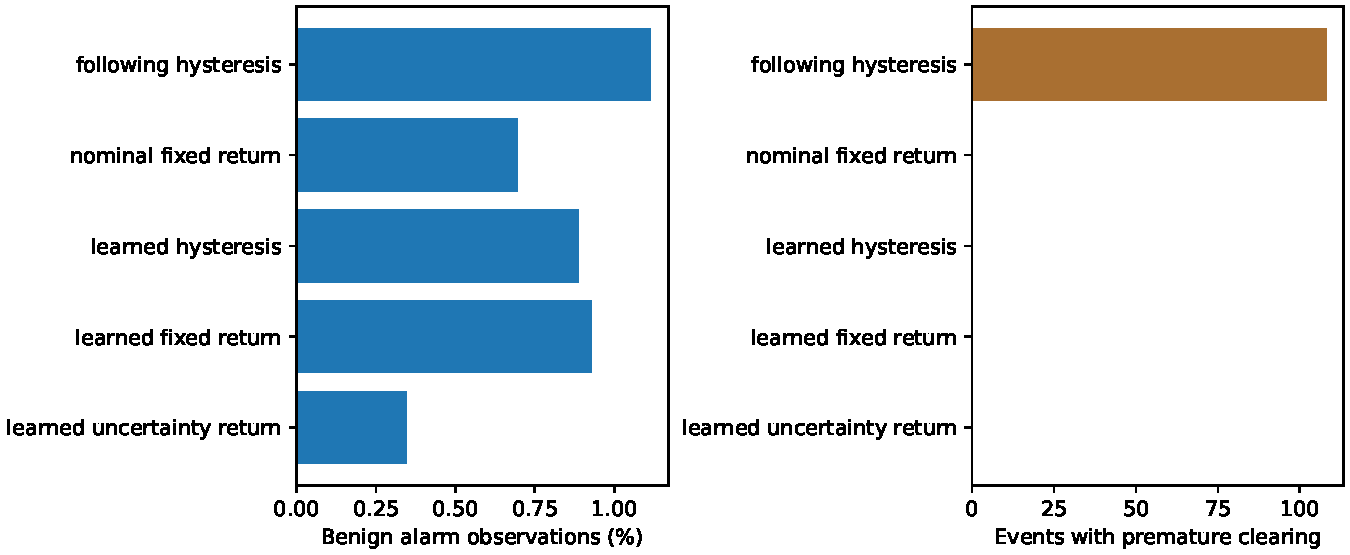
\includegraphics[width=\linewidth]{figures/recovery_tradeoff.pdf}
\caption{Benign alarm burden and premature clearing from saved pooled results. This figure must be read with Table~\ref{tab:all}: zero premature clearing does not imply that alarms eventually clear.}\label{fig:tradeoff}
\end{figure}

All 27 context-gap interventions were missed by the command-dependent methods under the declared unknown-history rule. Nominal-reference and paired-plant return times differed in 21 of 135 intervention episodes. The empirical allowance enclosed the complete eligible counterfactual-reference discrepancy in 189 of 216 episodes; this measured coverage does not justify a shifted-task guarantee.

One completed run took 229.20 s supervised wall time and 228.07 s worker CPU time. Sampled peak memory was 167.25 MiB; the worker's process-lifetime peak was 217.41 MiB. Output size was 118.32 MiB. The run stayed within 600 s wall, 300 s CPU, 1 GiB monitored memory and 256 MiB output caps. An earlier launch failed before worker initialization because process monitoring was blocked; it produced no scientific observations. Fourteen synthetic tests passed before freezing. Post-run verification passed 9,610 checks, including independent confusion-count and return calculations. Fit replay required matching the worker's single-thread BLAS settings; the failed default-thread check is retained.

\section{Discussion and limitations}
The proposed uncertainty allowance was intended to prevent premature clearance. In this experiment it instead made clearance impossible on two plants, while the same-threshold zero-allowance control retained all observed recovery benefits. The component has no demonstrated benefit here and should not be retained as an asserted contribution.

Stateful calibration can obscure this problem if assessed only by benign alarm time. A threshold may satisfy a finite normal-observation budget even though an eventual alarm enters an absorbing state. A normal-only feasibility check would have identified $b>\delta$ before attack evaluation. This check follows directly from the decision rule; it is a useful design constraint rather than a novel detection algorithm.

The same-plant counterfactual separates persistent attack effects from nominal-model error. Its availability is specific to simulation. In a physical system, such a trajectory would itself need estimation, uncertainty assessment and a defensible trust model. The clean commissioning assumption excludes poisoned initialization, and the approved-command assumption excludes coordinated compromise of that channel. Empirical ARX references can also miss nonlinear dynamics or benign disturbances that were absent from commissioning.

The experiment covers three specified plants and three analytic task families in one simulator. Noise seeds repeat physical conditions and do not create independent robot experiments. Plant factors co-vary, so subgroup differences cannot isolate the effect of lag, geometry or noise individually. The calibration allowance is empirical and the fresh task distribution differs from the calibration grid. No safety, real-time deployment or cross-robot generalization claim follows.

The comparison includes strong common-information controls and a recent threshold component, but it is not a paper-faithful benchmark against three recent detectors. Full-source admission of the closest recovery methods remains necessary for a broader original-method submission. The now-exposed conditions can diagnose the failure; they cannot confirm a subsequent redesign.

\section{Conclusion}
Reference proximity, command restoration and disappearance of attack-induced motion are distinct quantities. Explicit uncertainty bounds clarify when a return decision can be justified and when it is infeasible. In the frozen comparison, uncertainty-aware clearance reduced benign alarm counts but failed timely recovery; removing its allowance produced a stronger matched result. The supported design lesson is to establish clearance feasibility on normal operation and evaluate recovery against an independent target before interpreting nuisance-alarm reductions as an improvement.

\clearpage
\appendix
\section{Command families and reproducibility}\label{app:tasks}
For phase $\theta(s)$, amplitudes $a_1,a_2$ and offset $\phi$,
\begin{align}
q_1^c&=a_1\sin\theta+0.025\sin(2.3\theta),\\
q_2^c&=a_2\sin(\theta+\phi)+0.018\sin(1.7\theta).
\end{align}
Velocities are analytic derivatives, multiplied by the causal time-warp rate. Task E uses $\theta=0.63s$, amplitudes $(0.31,0.35)$ and $\phi=0.8$. Task F uses $\theta=0.38s+0.008s^2$, $(0.26,0.40)$ and $\phi=1.2$. Task G uses $\theta=0.83s+0.18\sin(0.31s)$, $(0.36,0.32)$ and $\phi=0.4$. Authorized slowdown retains accumulated phase delay; unauthorized slowdown rejoins the approved schedule on restoration.

Commissioning uses constant phase rates 0.35, 0.7 and 1.1, with amplitudes $(0.22+0.04i,0.34-0.025i)$ and phase offset $0.5+0.3i$, $i=0,1,2$. These episodes respectively use unchanged, authorized-offset and authorized-slowdown conditions. Calibration episode $i=0,\ldots,18$ uses phase rate $0.32+0.047i$, amplitudes $(0.23+0.012(i\bmod7),0.29+0.013(i\bmod9))$ and offset $0.4+0.06(i\bmod11)$, cycling through the same three benign conditions.

The local package retains full configuration, source/input hashes, training/calibration arrays, fitted coefficients, sealed scores, every outcome and resource receipt. It uses Python 3.12.15 and NumPy 1.26.4 in an isolated environment, with exact dependency and platform records. All figures and tables derive from saved artifacts. No raw benchmark recording was opened in this study. Table~\ref{tab:strata} preserves benign counts by plant; each denominator is 29,700.

\begin{table}[htbp]\centering\small
\caption{Benign alarm observations by plant.}\label{tab:strata}
\begin{tabular}{lrrr}\toprule
Method & Q1 & Q2 & Q3 \\\midrule
Persistence & 277 & 306 & 295 \\
ARX one-step & 239 & 272 & 281 \\
Following point & 217 & 275 & 302 \\
Following hysteresis & 368 & 322 & 303 \\
Nominal hysteresis & 131 & 334 & 324 \\
Nominal fixed return & 250 & 298 & 73 \\
Learned point & 216 & 254 & 349 \\
Learned hysteresis & 150 & 381 & 261 \\
Learned fixed return & 214 & 298 & 315 \\
Uncertainty return & 309 & 0 & 0 \\
Episode CP band & 0 & 0 & 0 \\
Matched no allowance & 140 & 0 & 0 \\
Matched no dwell & 20 & 0 & 0 \\
\bottomrule\end{tabular}

\end{table}

\section*{Declarations}
Muhammad Usman's supplied affiliation is COMSATS University Islamabad, Sahiwal Campus, Pakistan. Haiqa Mushtaq's affiliation, individual contributions, funding and competing-interest statements remain unconfirmed. Data are synthetic; code and results are retained in the local reproducibility package, with no public release.

\section*{Declaration of AI assistance}
Codex (OpenAI, GPT-6-based agent) assisted literature checks, study design, programming, experiment execution, verification and drafting. The exact serving build was unavailable. Tables and figures were computed from saved results using Python and Matplotlib. Review and approval by both named authors remain pending.

\begingroup\interlinepenalty=10000
\begin{thebibliography}{9}
\bibitem{casper} H. Kayan, R. Heartfield, O. Rana, P. Burnap, and C. Perera. CASPER: Context-Aware IoT Anomaly Detection System for Industrial Robotic Arms. \emph{ACM Transactions on Internet of Things}, 5(3), Article 18, 2024. \url{https://doi.org/10.1145/3670414}.
\bibitem{edge} H. Kayan, R. Heartfield, O. Rana, P. Burnap, and C. Perera. Real-Time Anomaly Detection for Industrial Robotic Arms Using Edge Computing. \emph{IEEE Internet of Things Journal}, 12(15):29696--29712, 2025. \url{https://doi.org/10.1109/JIOT.2025.3569780}.
\bibitem{fail} C. Xu et al. Can We Detect Failures Without Failure Data? Uncertainty-Aware Runtime Failure Detection for Imitation Learning Policies. \emph{Robotics: Science and Systems}, 2025. Author manuscript: \url{https://arxiv.org/abs/2503.08558}.
\bibitem{rescue} D. Ahmedt-Aristizabal, A. Khamis, M. A. Armin, and L. Petersson. RESCUE: Is This Alarm Worth Acting On? Counterfactual Evaluation of VLA Runtime Monitors. arXiv:2610.13516v1, 2026. \url{https://arxiv.org/abs/2610.13516}.
\bibitem{interval} J. Meseguer, V. Puig, T. Escobet, and J. Saludes. Observer gain effect in linear interval observer-based fault detection. \emph{Journal of Process Control}, 20(8):944--956, 2010. \url{https://doi.org/10.1016/j.jprocont.2010.06.017}.
\bibitem{rapio} I. Ahmed, A. Alharbi, J. Lu, A. Jaffar, and M. Bilal. Robust Adaptive Propagated Interval Observer for Actuator Fault Diagnosis in Underactuated AUVs. \emph{Journal of Marine Science and Engineering}, 14(15):1445, 2026. \url{https://doi.org/10.3390/jmse14151445}.
\bibitem{kaisar} H. Kaisar, M. Rehan, I. Ahmed, M. Bilal, and M. Khalid. A Digital Twin-Based Cybersecurity Architecture for FDI Anomaly Detection and Isolation in Next Generation Robotic Vehicles. \emph{IEEE Open Journal of the Communications Society}, 7:12709--12728, 2026. \url{https://doi.org/10.1109/OJCOMS.2026.3739185}.
\end{thebibliography}\endgroup
\end{document}
